\documentclass[a4paper,10pt,notitlepage]{report}
\usepackage[utf8]{inputenc}
\usepackage{authblk}
\usepackage{geometry}
\usepackage{graphicx}
\usepackage{float}
\usepackage{cite}
\usepackage{caption}
\usepackage{subcaption}
\usepackage{hyperref}


\pdfinfo{%
  /Title    ()
  /Author   (Rafał Sikora)
}

%additional symbols
\newcommand{\Pom}{I$\!$P}             % gives pomeron symbol
\newcommand{\Reg}{I$\!$R}               % gives pomeron symbol
\newcommand{\DPE}{D\Pom E}
\newcommand{\Pomeron}{\Pom omeron}

%chapter heading
\makeatletter
\renewcommand{\@makechapterhead}[1]{%
 \vspace*{18\p@}%
  {\parindent \z@ \raggedright
%     \LARGE \bfseries \thechapter. #1\par\nobreak
%     \vskip 40\p@
      \Huge \bfseries \thechapter. #1\par\nobreak
      \vskip 40\p@
  }}
\makeatother


% Title Page
\title{\textbf{Measurement of Central Exclusive Production\\with Roman Pot detectors in diffractive proton-proton interactions at~$\sqrt{s}=$~200~GeV}\vspace*{10pt}}
\author[1]{Leszek Adamczyk}
\author[1]{Łukasz Fulek}
\author[1]{Mariusz Przybycień}
\author[2]{Wlodek Guryn}
\author[1]{\underline{Rafał Sikora}}
\affil[1]{AGH University of Science and Technology, FPACS, Kraków, Poland}
\affil[2]{Brookhaven National Laboratory, Upton, NY, USA}
% \affil[$\dag$]{Primary author}

\setcounter{Maxaffil}{0}
\renewcommand\Affilfont{\itshape\small}
\renewcommand{\bibname}{References}

\begin{document}

\begin{center}
\begin{minipage}[c]{0.12\linewidth}%
\vspace{5.5pt}\textbf{\LARGE{of the}}
\end{minipage}
\begin{minipage}[c]{0.15\linewidth}%
\hspace*{-8pt}
\includegraphics[width=\linewidth]{graphics/STAR_logo.pdf}
\end{minipage}~
\begin{minipage}[c]{0.24\linewidth}%
\vspace{9pt}\hspace*{-8pt}\textbf{\LARGE{Experiment}}
\end{minipage}\\[-50pt]
\textbf{\LARGE{Analysis Note}}

\vspace*{150pt}
\begin{minipage}{\linewidth}
\maketitle
\begin{abstract}
In this note we present analysis of the Central Exclusive Production process using data from proton-proton collisions collected in 2015. This data was collected using the Roman Pot detectors which ensured efficient triggering and measuring diffractively scattered protons. We describe all intermediate stages of analysis involving extraction of the acceptance and effciency corrections, comparison of data with Monte Carlo simulations of detector response, and study of systematic uncertainties. Finally, we show the physics outcome of the analysis.
\end{abstract}
\thispagestyle{empty}
\end{minipage}

\vspace{50pt}

 \Huge{\textbf{\textit{DRAFT}}}
\end{center}


\clearpage
\thispagestyle{empty}
\newgeometry{hmargin={2cm, 2cm}, height=10.0in}
\tableofcontents


%% =====  INTRODUCTION ====
%%===========================================================%%
%%                                                           %%
%%                       INTRODUCTION                        %%
%%                                                           %%
%%===========================================================%%


\chapter{Introduction}\label{chap:introduction}

% * ** *** **** ***** ****** ******* S E C T I O N ******* ****** ***** **** *** ** *
\section{Central Exclusive Production}
The Central Exclusive Production (CEP) takes place when interacting particles form in the mid-rapidity region a state (``central production'') whose all constituents/decay products are measured in the detector (``exclusive''). The initial state particles can either dissociate, excite or stay intact. The latter case of CEP in proton-proton collisions can be written as
\begin{equation}\label{eq:cep}%
p~~+~~p~~~\rightarrow~~~p~~+~~X~~+~~p
\end{equation}
and depicted as in Fig.~\ref{fig:eta_phi}. Mass and rapidity of state $X$ is given by\\[-10pt]
\begin{tabulary}{\textwidth}{CCR}
\begin{equation}\label{eq:mass_X}
M_{X} = \sqrt{s\Big(\xi_{1}\xi_{2}\sin^{2}{(\alpha/2)}-(1-\xi_{1}-\xi_{2})\cos^{2}{(\alpha/2)}\Big)} \stackrel{\alpha=\pi}{=} \sqrt{s\xi_{1}\xi_{2}},
\end{equation}~~~~~~~~~~~~~~~~ & ~~ & ~~~~~~
\begin{equation}\label{eq:rapidity_X}
y_{X} = \frac{1}{2}\ln{\frac{\xi_{1}}{\xi_{2}}},
\end{equation}~~~~~~~~
\end{tabulary}\\[-10pt]
where $\alpha$ is angle between scattered protons and $\xi=(p_{0}-p)/p_{0}$ is the fractional momentum loss of proton.\vspace{-5pt}

% * ** *** **** ***** ****** ******* S E C T I O N ******* ****** ***** **** *** ** *
\section{Double \Pomeron\  Exchange}\label{sec:DPE}
Reaction from Eq.~\ref{eq:cep} can exhibit purely electromagnetic ($\gamma$-$\gamma$), mixed ($\gamma$-$\mathcal{O}$) or purely strong nature ($\mathcal{O}$-$\mathcal{O}$). The last type is dominant at RHIC energies. It is characterized by the lack of hard scale (if protons are scattered at small angles), therefore perturbative QCD cannot be applied and Regge theory~\cite{IntroductionToRegge} is used instead. An object $\mathcal{O}$ does not have unequivocal QCD representation - in Regge formalism it is the so-called ``trajectory`` (\Reg eggeon, \Reg). \Reg eggeon with quantum numbers of vacuum is called ''\Pomeron`` (\Pom) and \Pom-\Pom\ reaction (Fig.~\ref{fig:DPE}) is called ''Double \Pomeron\  Exchange``. %

%---------------------------
\begin{figure}[b!]
\centering
\parbox{0.475\textwidth}{%
  \centering%
  \hspace*{-10pt}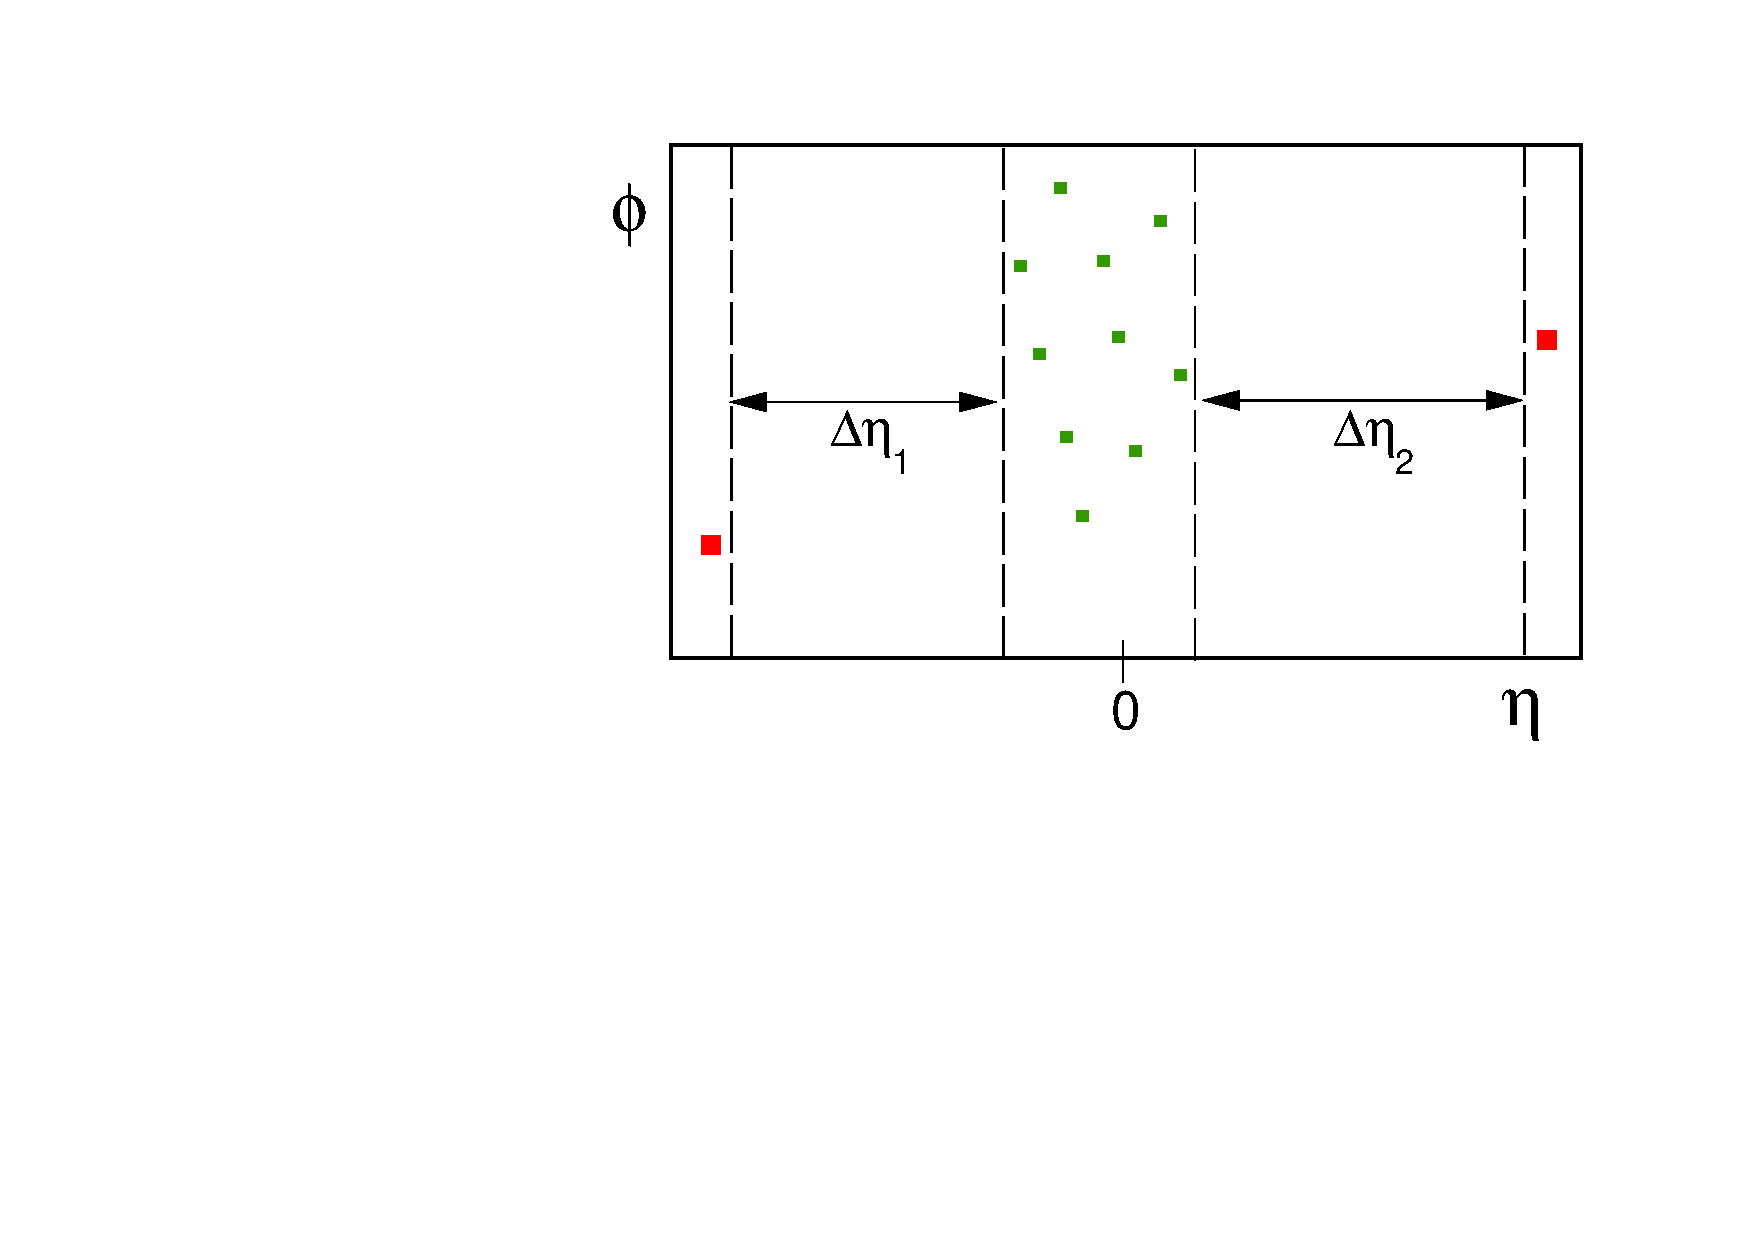
\includegraphics[width=1.1\linewidth]{graphics/introduction/eta_phi.pdf}\vspace*{-10pt}%
  \caption{Central Exclusive Production in $\eta$-$\phi$ space.\\}%
  \label{fig:eta_phi}%
}
\quad
\parbox{0.475\textwidth}{%
  \centering%
  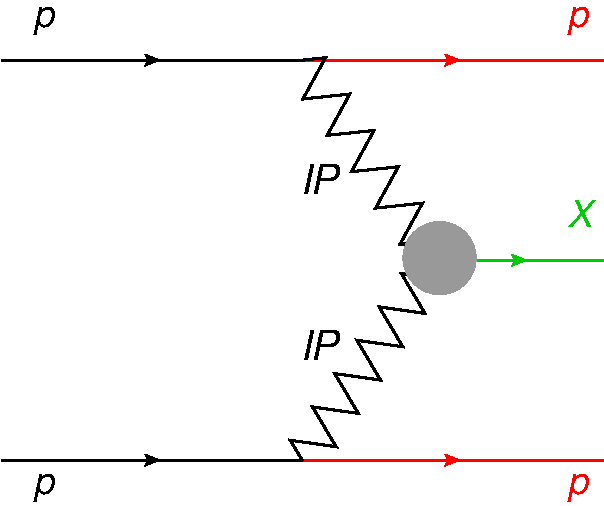
\includegraphics[width=0.64\linewidth]{graphics/introduction/DPE.pdf}%
  \caption{Diagram of D\Pom E process.\\}%
  \label{fig:DPE}%
}\vspace*{-25pt}
\end{figure}
%---------------------------

Processes involing \Pomeron\  exchange are referred as diffraction due to cross-section in scattering angle resembling similar shape to instesity pattern of diffracted light. For low values of Mandelstam $t$ (small scattering angles) cross-section takes exponential form\vspace{-10pt}
\begin{equation}
 \frac{d\sigma_{a}}{d|t|} \propto e^{-B|t|},
\end{equation}%
where the slope parameter $B$ reflects the size of target at which \Pomeron s scatter.

Diffractive events have specific property of the ''rapidity gap`` which is an angular region free of hadrons. In \DPE\ two such gaps are present, marked in Fig.~\ref{fig:eta_phi} as $\Delta\eta_{1}$ and $\Delta\eta_{2}$.%

\DPE\ is a spin-parity filter - from the fact that scattered particles have all quantum numbers unchanged after the interaction, central states must satisfy
\begin{equation}\label{eq:DPE_IGJPC}
 I^{G}J^{PC}=0^{+}\textrm{even}^{++}.
\end{equation}%

The lowest order QCD picture of the \Pomeron\ is a pair of oppositely colored gluons (colour singlet). This fact makes the \DPE\ recognized as the gluon-rich environment process which should enhance production of the bound states of gluons (''glueballs``) or hybrid mesons.

For detailed introduction to the topic of diffraction see \cite{pomeronAndQCD,barone}.\vspace*{-20pt}

% * ** *** **** ***** ****** ******* S E C T I O N ******* ****** ***** **** *** ** *
\section{Physics motivation for the measurement}
STAR collected in 2015 large dataset dedicated for the measurement of the Central Diffraction (\DPE\ in particular). Since that year the experiment was enriched with Roman Pot Phase II* subsystem and thus gained possibility of detection of forward protons. It enabled studies of properties of the central state with respect to observables related to exchanged \Pomeron s. No such measurement was performed before at that high c.m.s. energy ($\sqrt{s}=200$~GeV, contamination from \Reggeon\ exchanges is small) which makes it particularly attractive. A list of physics issues that can be covered with the study described in this note is briefly introduced below.%
%
\subsection{\DPE\ differential cross-sections, mass spectrum}

As stated in Sec.~\ref{sec:DPE} \DPE\ is a soft process whose theoretical description is done mainly using phenomenological tools, thus measurement of differential cross-sections is needed to verify various production models.

The main focus is put on the simplest state (and most numerously) produced in \DPE, namely a pair of oppositely charged pions, $\pi^{+}\pi^{-}$. It can be formed either in a non-resonant or resonant mechanism. In the first case the $\pi^{+}\pi^{-}$ continuum is formed by the exchange of the off-shell pion between \Pomeron s. Currently there are two models of this reaction on the market~\cite{LSmodel,LSmodel2},~\cite{DurhamModel}. In the second case the \Pomeron s directly couple into resonance (e.g. $f_{2}(1270)$), which then decays to $\pi^{+}\pi^{-}$. Attempts to calculate cross-section for this production mechanism are presented in \cite{LSmodel2} and \cite{Schicker}.

Understanding of the mass spectrum in $\pi^{+}\pi^{-}$ channel is important to learn about relative contribution from continuum and resonant production, as well as relative production of resonances. Recognition of resonant states may indicate candidates for low-mass glueballs of $J^{PC}=0^{++}$, however presence of underlaying scalar $q\bar{q}$ states makes this task challenging.

Other channels, like $K^{+}K^{-}$, are also of great interest. Comparison of the cross-sections for production of $\pi^{+}\pi^{-}$ and $K^{+}K^{-}$ gives information about strength of the \Pomeron\ coupling to different quark flavors. Also, structures in $d\sigma/dm$ can be easier attributed to resonances by measuring more than one channel and known branching ratios thereof.

Detection of intact protons scattered at very small angle with respect to the beamline enables determination of the reaction plane which makes the Partial Wave Analysis (PWA) possible. It also allows to look at the the cross-sections more differentially, especially with respect to properties of exchanged \Pomeron s, like carried squared four-momentum $t$, azimuthal separation of the \Pomeron s in the transverse plane $\Delta\varphi$ or relative momentum of \Pomeron s $\Delta p_{T}$. The last quantity was proposed to distinguish pure $q\bar{q}$ states from these with gluonic content~\cite{DPtFilter}.

\subsection{Absorption effects}

One can imagine in diagram in Fig.~\ref{fig:DPE} additional soft lines e.g. between protons in the initial state or one of \Pomeron s and final state proton. These so-called rescattering effects (or absorption effects) lead to production of hadrons other than these belonging to central state $X$ and the diffractive signature of an event in form of rapidity gap is no longer present. Measurement of the probability that the state $X$ will remain exclusive and forward protons will remain intact, in other words the rapidity gap survival probability $S^{2}$, would be valuable ingredient for development of absorption models.

\subsection{Size of interaction region}

From the measurement of protons in Roman Pots one is able to reconstruct squared four-momenta transferred in proton-\Pomeron\ vertices and determine the differential cross-section $d\sigma/d|t|$. Fit of exponent allows to extract the slope parameter $B$, which may depend on the \Pomeron-\Pomeron\ c.m.s. energy, or in other words on the mass of diffractive system $X$. Knowledge on the slope parameter gives insight to the volume and distribution of \Pomeron s inside proton.

%% =====  DATASET ====
%%===========================================================%%
%%                                                           %%
%%                          DATASET                          %%
%%                                                           %%
%%===========================================================%%


\chapter{Data set}\label{chap:dataset}

\section{Trigger}\label{seq:trigger}

The main trigger designed for studies of Central Diffraction in run 15 was RP\_CPT2. It was formed of the following conditions combined by logical AND (\&\&):
\begin{enumerate}
 \item \textbf{(ET \&\& !IT) $||$ (!ET \&\& IT)} = signal in at least one RP on each side of the STAR central detector - to ensure presence of two forward-scattered protons; a veto was imposed on simultaneous signal in RPs above and below the beamline, which might have originated either from proton dissociation, or pile-up event, or beam halo proton etc.,
 \item \textbf{!BBCE \&\& !BBCW \&\& !ZDCE \&\& !ZDCW} = veto on any signal in small BBC tiles or ZDCs on any side of STAR central detector - such requirement is in accordance with the double-gap topology of CEP events, it mostly filtered out CEP events with parallel pile-up event(s),
 \item \textbf{TOF$\geq$2} = at least 2 hits in TOF - aim of this condition was to ensure activity in the mid-rapidity; since the lowest multiplicity allowed in CEP is 2, that was the lower threshold of L0 TOF multiplicity.
\end{enumerate}%
This trigger was running with an average prescale of 5 and average DAQ rate of 250~Hz, which allowed to collect in total about 560~M events corresponding to 16.5~pb$^{-1}$ of integrated luminosity.  More information about number of events per run, rates etc. can be found under link provided in Ref.~\cite{onlineRpTriggersMonitoring}, which contains selected data from STAR run log~\cite{RunLog}. Luminosity data used in this analysis comes from Ref.~\cite{Luminosity}.

All RP triggers which were intended for usage in diffractive physics analyses or efficiency studies are listed in Tab.~\ref{tab:triggers}. Components used in definitions of these triggers are outlined in Fig.~\ref{fig:triggerBits}. Detailed explanation of all trigger bits can be found in Refs.~\cite{RpTriggers,RpTriggers2}. Explanation of naming convention in Roman Pot system can be found in Ref.~\cite{Labeling}.

\begin{figure}[h]
 \centering%
 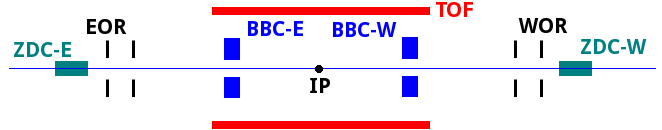
\includegraphics[width=0.71\linewidth]{graphics/dataset/bits.png}%
 \caption{Sketch of the trigger components used in definitions of diffractive triggers in run 15.}\label{fig:triggerBits}%
 \end{figure}


\begin{table}[hb!]\centering
 \begin{tabular}{l|c|c|c}%\hline
 \textbf{\specialcell{Trigger\\name}} &  \textbf{Definition} &  \textbf{Events [M]} &  \textbf{Comment} \\ \hline
 RP\_CP & {EOR \&\& WOR} & 73.3 & \specialcell{Loose trigger (mostly elastic events) designed\\for monitoring/trigger efficiency study}\\ \hline
 RP\_CPT & {\specialcell{\specialcell{EOR \&\& WOR\\ \&\& !BBCE \&\& !BBCW} \\ \specialcell{\&\& !ZDCE \&\& !ZDCW} \\ \&\& TOF$\geq$1}} & 38.9 & \specialcell{Intended to be main CEP trigger (later\\switched to RP\_CPT2 due to large prescale)}\\ \hline
 RP\_CPT2 & {\specialcell{\specialcell{(ET \&\& !IT) $||$ (!ET \&\& IT) \\ \&\& !BBCE \&\& !BBCW} \\ \specialcell{\&\& !ZDCE \&\& !ZDCW} \\ \&\& TOF$\geq$2}} & 556.5 & \specialcell{Main CEP trigger\\Note: On Apr 14 added upper TOF limit (10)} \\ \hline
 RP\_CPX & {\specialcell{\specialcell{IT\\ \&\& !BBCE \&\& !BBCW} \\ \specialcell{\&\& !ZDCE \&\& !ZDCW} \\ \&\& TOF$\geq$2}} & 40.1 & \specialcell{The same as RP\_CPT2\\but only IT configuration}\\ \hline
 RP\_CPEI & {\specialcell{\specialcell{ET \&\& IT\\ \&\& !BBCE \&\& !BBCW} \\ \specialcell{\&\& !ZDCE \&\& !ZDCW} \\ \&\& TOF$\geq$2}} & 15.6 & \specialcell{Control trigger for CPT2 to estimate\\ effect of !(ET \&\& IT) veto } %\\ \hline
\end{tabular}\caption{Central Diffraction physics triggers and control triggers involving Roman Pot detectors in run 15.}\label{tab:triggers}
\end{table}


\section{Reconstruction software}\label{sec:recoSoftware}

Raw data was processed with STAR libraries in versions SL17f. All four trigger datasets were processed: production\_pp200trans\_2015, production\_pp200long2\_2015, production\_pp200long3\_2015 and production\_pp200long\_2015 (see~\cite{ProductionList}).

The following BFC options were used in the reconstruction:\vspace{-5pt}
\begin{verbatim}
DbV20160418,pp2015c,btof,mtd,mtdCalib,pp2pp,-beamline,beamline3D,useBTOFmatchOnly,VFStoreX,
fmsDat,fmsPoint,fpsDat,BEmcChkStat,-evout,CorrX,OSpaceZ2,OGridLeak3D,-hitfilt
\end{verbatim}
Main attention should be put on option \textbf{useBTOFmatchOnly} which forced vertexing algorithm to form vertices only from the global TPC tracks which are matched with hits in the TOF system. This solution was found to yield significantly larger signal reconstruction efficiency (vertexing efficiency) and better resolutions. The study which lead to above conclusions, presented in Ref.~\cite{RevertexingProposal}, was performed on the same dataset processed with older libraries SL15k (without useBTOFmatchOnly option).



\section{Data format}\label{sec:dataFormat}

The analyzed data was stored in ROOT files in the picoDST format which was in large part a skimmed MuDST (standard STAR format). The picoDST format was introduced in Ref.~\cite{PicoDstDescription}. PicoDST description files (C++ headers etc.) can be found in the analysis code repository~\cite{AnalysisCodeRepo}.

\section{Bad runs}\label{sec:badRuns}

Analysis of CEP was performed on the data from runs with completion status ``Successful'' in the STAR run log. However, based on additional requirements explained below, some runs were omitted from analysis.

\subsection{RP distance from the beamline}

16065025
16065026
16065027
16065028
16072057
16072058
16077055
16083006
16083007
16106031

%---------------------------
\begin{figure}[hb]
\centering
\parbox{0.4\textwidth}{
  \centering
  \begin{subfigure}[b]{\linewidth}{
                \subcaptionbox{\label{fig:positionHistograms}}{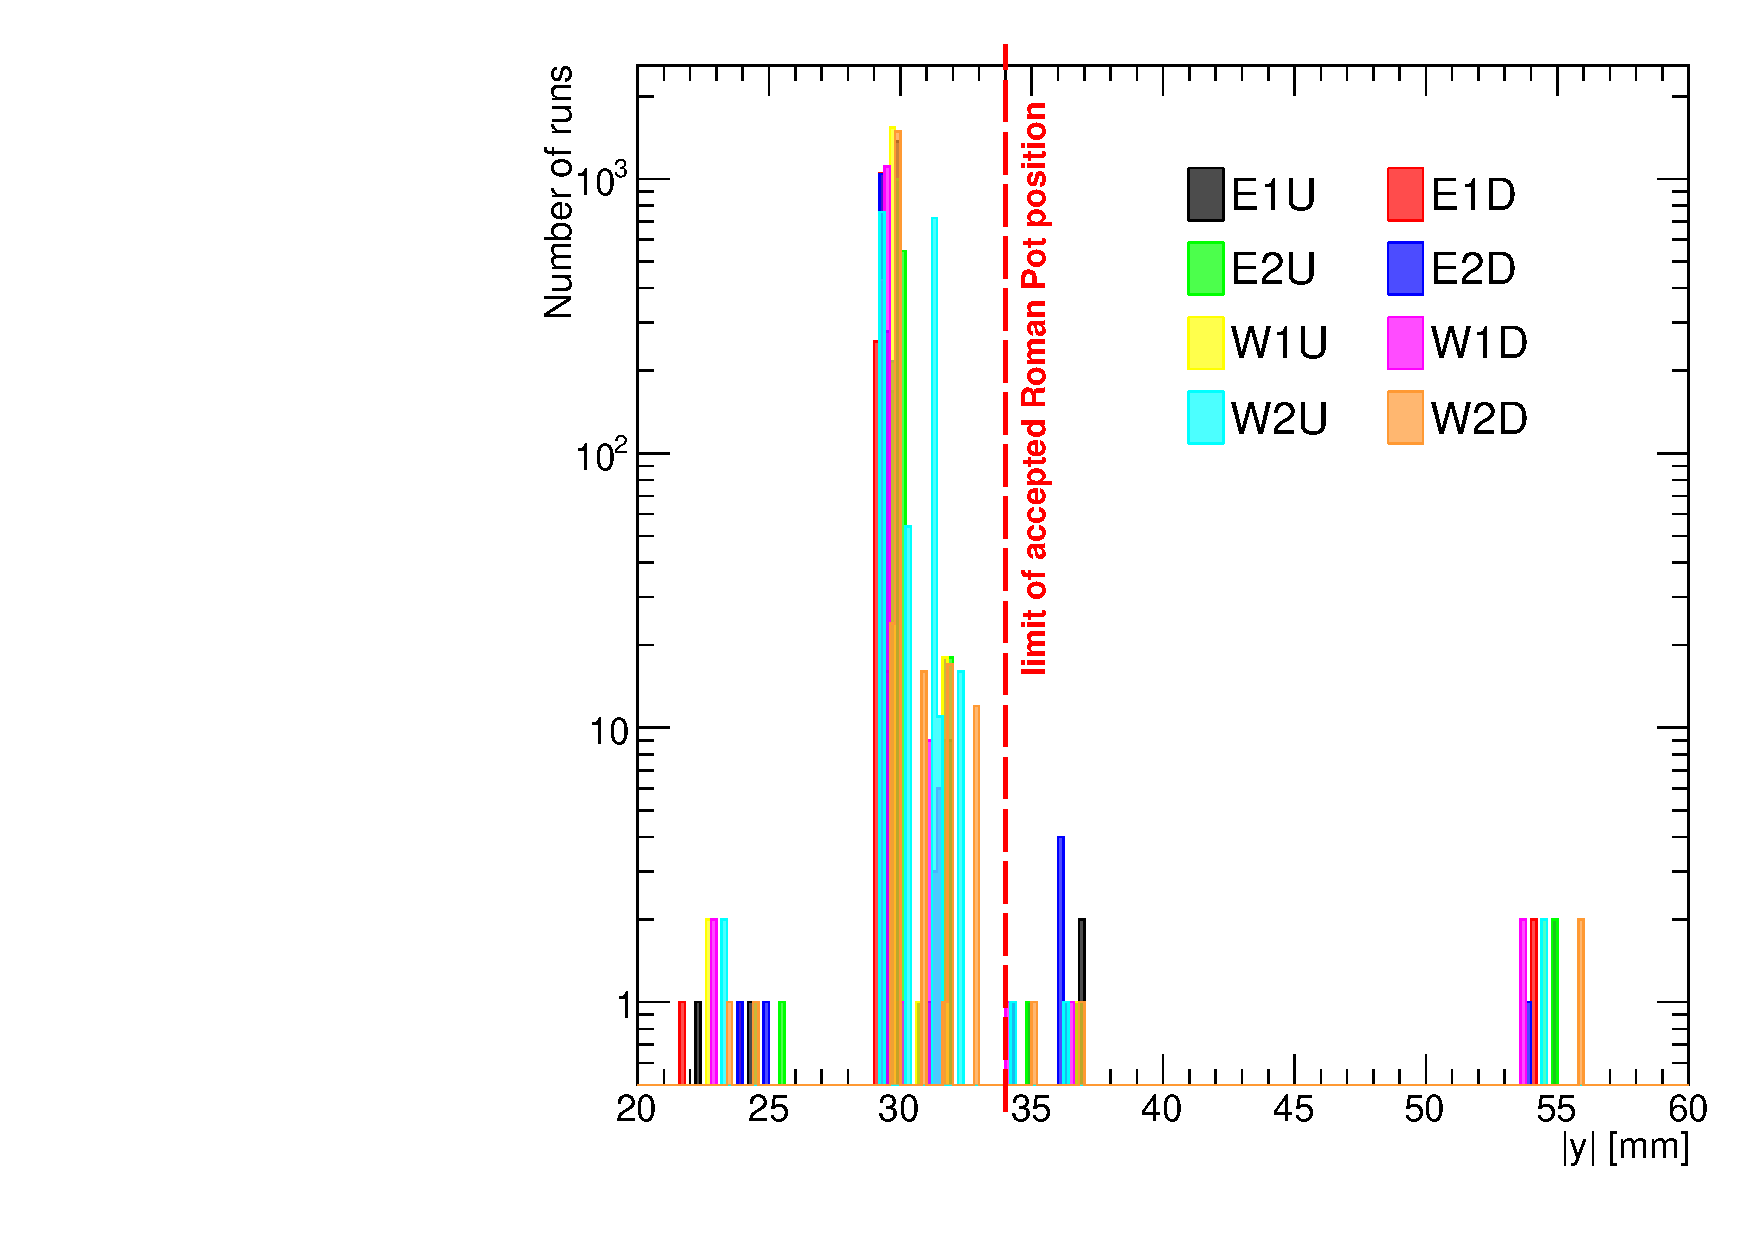
\includegraphics[width=\linewidth]{graphics/dataset/positionHistograms.pdf}}}
  \end{subfigure}
}
\quad
\parbox{0.545\textwidth}{
  \centering
  \begin{subfigure}[b]{\linewidth}{
                \subcaptionbox{\label{fig:positionVsRunGraph}}{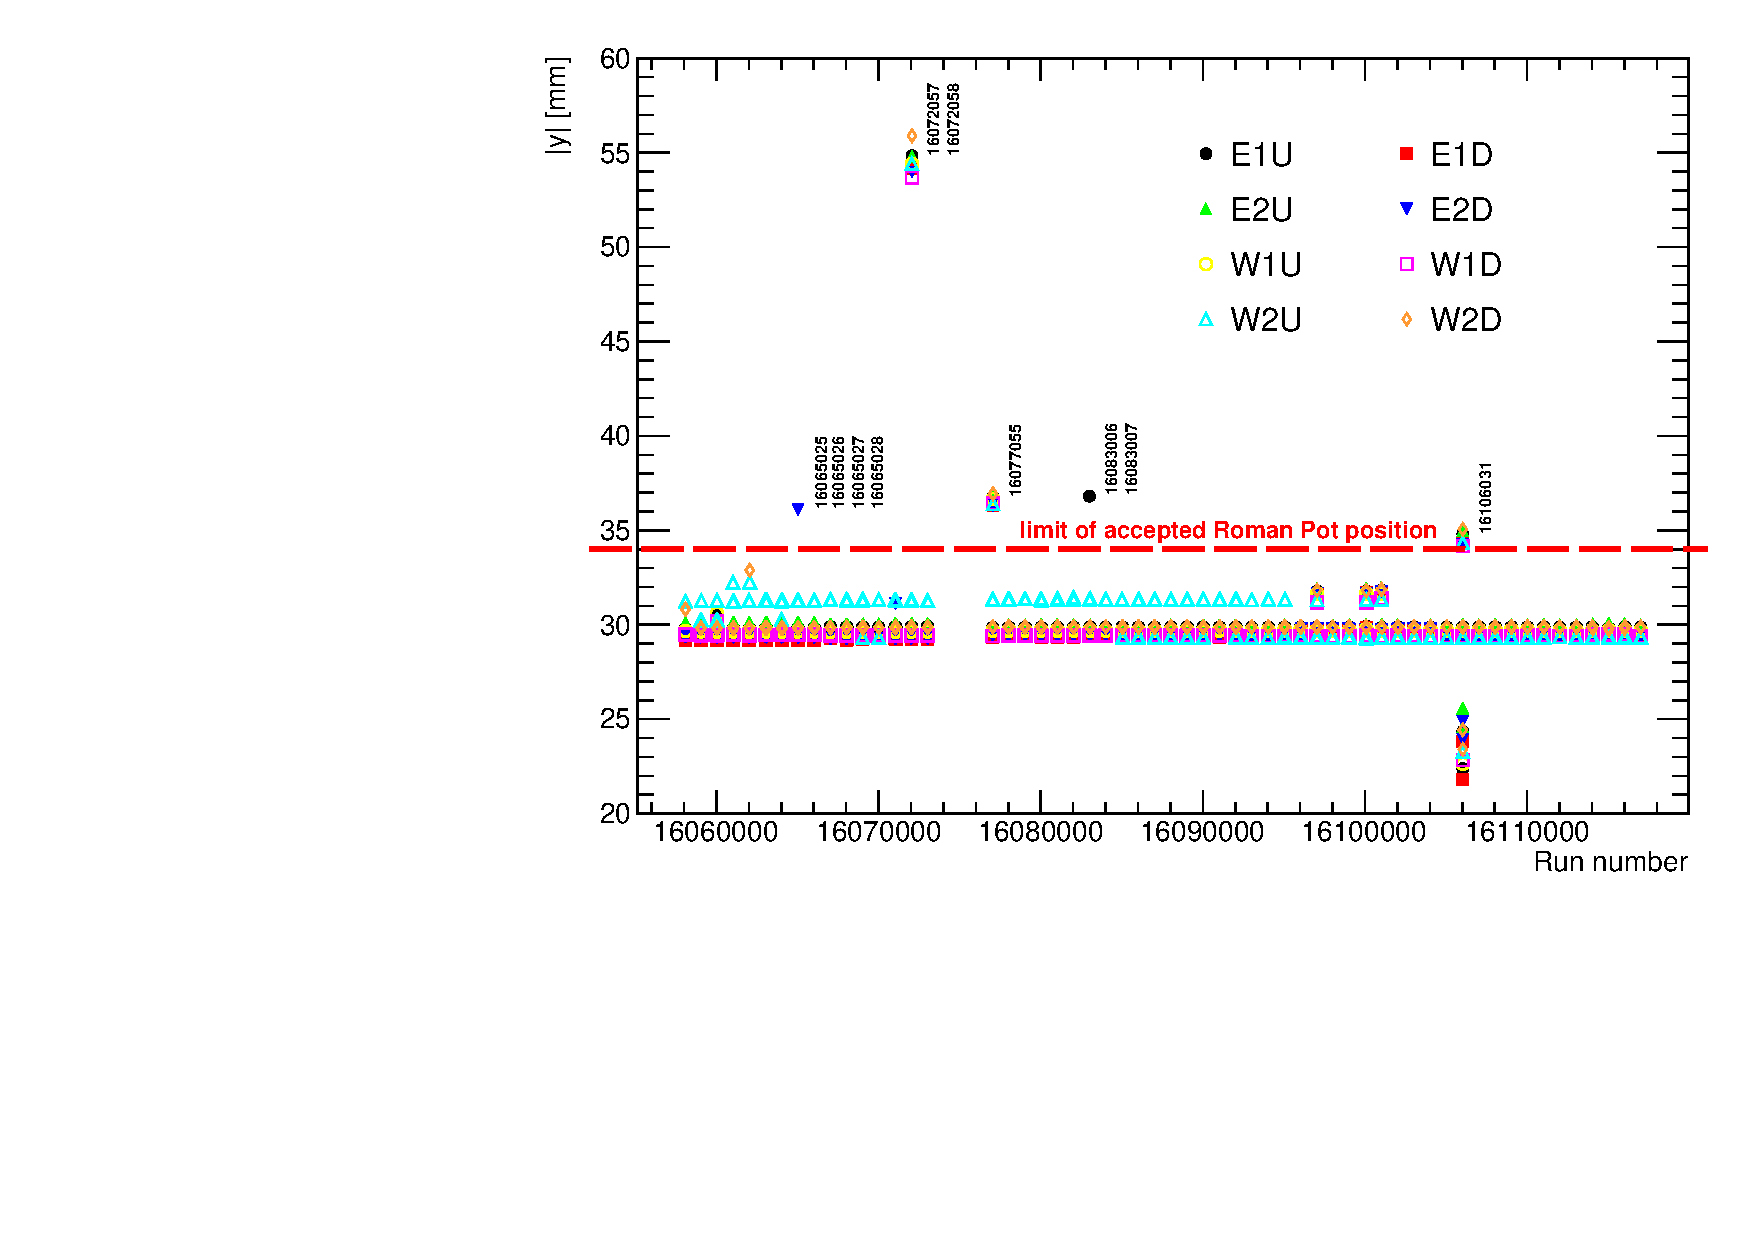
\includegraphics[width=\linewidth]{graphics/dataset/positionVsRunGraph.pdf}}}
  \end{subfigure}
}%
\caption[Beam-detector distance of the Roman Pots in run 15.]{Histogram of beam-detector distance $|y|$ (\ref{fig:positionHistograms}) and graph showing run-dependence of $|y|$ (\ref{fig:positionVsRunGraph}) for all Roman Pots.}%\label{fig:xy_recoEff}
\end{figure}
%---------------------------



% %% ===== DODATKI ===== ------------
% \begin{appendices}
% \input{Appendix_RunList.tex}
% \input{Appendix_tDistributions.tex}
% \input{Appendix_AngularBeamDivergence.tex}
% \input{Appendix_BunchProfiles.tex}
% \end{appendices}



\bibliography{references.bib}{}
\bibliographystyle{utphys}
\addcontentsline{toc}{chapter}{References}

\end{document}          
